% !TEX TS-program = lualatexmk
% !TEX parameter =  --shell-escape
\documentclass[benediction_assumption_la_en.tex]{subfiles}

\ifcsname preamble@file\endcsname
  \setcounter{page}{\getpagerefnumber{M-benediction_assumption_la_en_exposition}}
\fi

\begin{document}

\chapter*{AT EXPOSITION.}
\addcontentsline{toc}{chapter}{At Exposition}

\textes{o_salutaris_la_en}

\vspace{0.5\baselineskip}
\rubrique{The cantors intone until the asterisk or the quarter bar.}

\smalltitle{On Major Feasts.}

\rubrique{Melody of the hymn \normaltext{Verbum supérnum,} from Lauds of Corpus Christi.}

\gscore[]{8.}{o_salutaris_mode_8}

\smalltitle{On Sundays \textit{per annum} and until Ash Wednesday.}

\rubrique{Alternate medieval melody restored in the Vatican Edition.}

\gscore[]{7.}{hy_o_salutaris_mode_7}

\smalltitle{In Advent and Lent.}

\rubrique{\begin{enpars}\normaltext{O Salutáris VI,} from \normaltext{Cantus Selecti,} 1957; melody of \normaltext{Cónditor alme sidérum} from the office of the Most Holy Redeemer.\end{enpars}}

%%why is spacebeneathtext larger
%%aha it stretches when the pdf is inserted
%keep explicit newpage

\gscore[]{4.}{hy_o_salutaris_vi_cantus_selecti_solesmes}

\smalltitle{In Paschal Time.}

\rubrique{\normaltext{O Salutáris III,} in the \normaltext{Liber antiphonarius,} 1949. Melody of the hymn \normaltext{Beáta nobis gaúdia} from Lauds of Pentecost.}

%%why is  the text above so close? just why?!
%%for now solution is explicit vspace
\vspace{0.5\baselineskip}

\gscore[]{1.}{hy_o_salutaris_hostia_liber_antiphonarius_3_solesmes}

\newpage

\smalltitle{On Weekdays \textit{ per annum.}}

{\centering{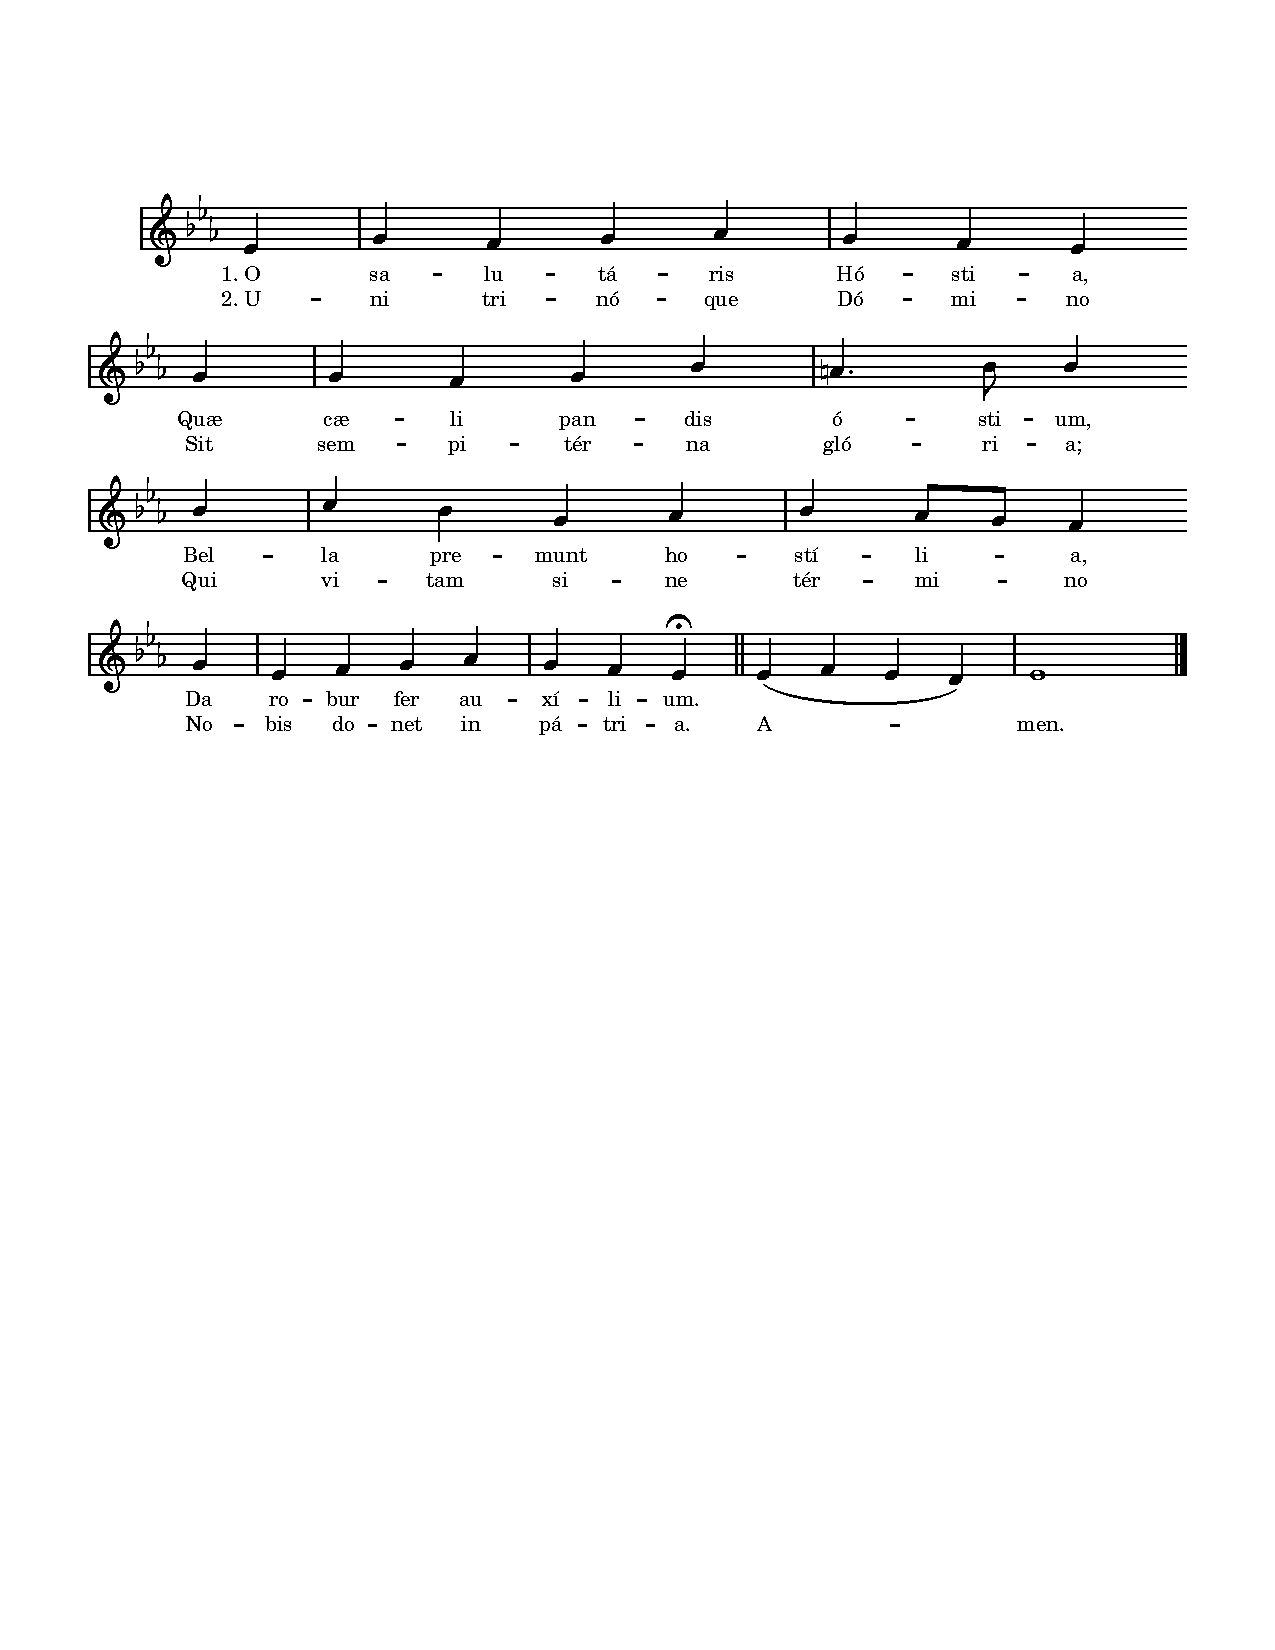
\includegraphics[scale=0.75,keepaspectratio]{O_salutaris_Hostia_Duguet_melody_cropped}\par}}

\rubrique{
\begin{enpars}
 Afterwards, on weekdays, confessions are ordinarily heard; otherwise, devotions follow immediately according to the day, the month, or the occasion.\end{enpars}}

\end{document}